% Mortgage Denial Models -- HMDA 2024
% Build the figures, tables and numbers first:   python report/build_latex.py
% Then compile (twice for references):          tectonic main.tex     (or: latexmk -pdf main.tex)
\documentclass[11pt,a4paper]{article}

\usepackage[T1]{fontenc}
\usepackage[utf8]{inputenc}
\usepackage{lmodern}
\usepackage{microtype}
\usepackage[a4paper,left=26mm,right=26mm,top=26mm,bottom=28mm]{geometry}
\usepackage{amsmath,amssymb,bm}
\usepackage{booktabs,array,multirow}
\usepackage{graphicx}
\usepackage{float}
\usepackage{xcolor}
\usepackage{caption}
\usepackage{enumitem}
\usepackage{fancyhdr}
\usepackage{titlesec}
\usepackage{tikz}
\usetikzlibrary{positioning,arrows.meta}
\usepackage[hidelinks]{hyperref}

\definecolor{navy}{HTML}{1D4F8C}
\definecolor{okgreen}{HTML}{0B7A4B}
\definecolor{badred}{HTML}{B3261E}

\newcommand{\NRows}{3\,208\,974}
\newcommand{\NTrain}{2\,567\,179}
\newcommand{\NTest}{641\,795}
\newcommand{\DenialRate}{8.83\%}
\newcommand{\RateConv}{7.70\%}
\newcommand{\RateFHA}{12.53\%}
\newcommand{\RateVA}{8.17\%}
\newcommand{\RateUSDA}{12.20\%}
\newcommand{\AROC}{0.735}
\newcommand{\APR}{0.426}
\newcommand{\CROC}{0.763}
\newcommand{\CPR}{0.478}
\newcommand{\GROC}{0.795}
\newcommand{\GPR}{0.524}
\newcommand{\EGain}{0.012}
\newcommand{\BasePR}{0.088}
\newcommand{\Gap}{0.046}
\newcommand{\DtiConvLow}{5.4\%}
\newcommand{\DtiConvHigh}{65\%}
\newcommand{\DtiFhaMid}{12\%}
\newcommand{\DtiFhaHigh}{98\%}
\newcommand{\DtiVaMid}{7.5\%}
\newcommand{\DtiVaHigh}{40\%}
\newcommand{\DtiUsdaLow}{9\%}
\newcommand{\DtiUsdaMid}{24\%}
\newcommand{\ClConvLow}{6.9\%}
\newcommand{\ClConvHigh}{15.7\%}
\newcommand{\ClVaLow}{7.9\%}
\newcommand{\ClVaHigh}{27\%}
\newcommand{\ORDtiHigh}{89}
\newcommand{\ORDtiMid}{4.2}
\newcommand{\ORVA}{0.36}
\newcommand{\ORCltvHigh}{2.31}
\newcommand{\ORIncome}{3.9}
\newcommand{\FitASk}{6}
\newcommand{\FitASp}{15}
\newcommand{\FitCSk}{60}
\newcommand{\FitCSp}{89}
\newcommand{\SparkIterC}{200}


% ---- layout
\setlength{\parindent}{0pt}
\setlength{\parskip}{0.55em}
\renewcommand{\arraystretch}{1.15}
\captionsetup{font=small,labelfont=bf,labelsep=period,justification=raggedright,singlelinecheck=false,skip=6pt}
\setlist{itemsep=2pt,topsep=3pt}
\graphicspath{{figures/}}
\setcounter{secnumdepth}{2}
\titleformat{\section}{\Large\bfseries}{\thesection}{0.7em}{}
\titleformat{\subsection}{\large\bfseries}{\thesubsection}{0.6em}{}
\titlespacing*{\section}{0pt}{2.2ex plus 0.5ex}{1ex}
\titlespacing*{\subsection}{0pt}{1.8ex plus 0.4ex}{0.6ex}
\pagestyle{fancy}
\fancyhf{}
\fancyhead[L]{\small\itshape Mortgage Denial Models}
\fancyhead[R]{\small\itshape HMDA 2024}
\fancyfoot[C]{\small\thepage}
\renewcommand{\headrulewidth}{0.3pt}
\setlength{\headheight}{14pt}

\newcommand{\DTI}{\textsc{dti}}
\newcommand{\CLTV}{\textsc{cltv}}
\newcommand{\code}[1]{\texttt{\small #1}}
\newcommand{\pr}{\operatorname{Pr}}
\newcommand{\indic}{\mathbf{1}}
\newcommand{\Var}{\operatorname{Var}}
\DeclareMathOperator*{\argmin}{arg\,min}

\hypersetup{pdftitle={Mortgage Denial Models},pdfauthor={},pdfsubject={HMDA 2024 logistic regression}}

\begin{document}

% ------------------------------------------------------------------ title
\begin{center}
  {\bfseries\huge Mortgage Denial Models}\\[1.6ex]
  {\large\itshape Models that predict if a lender denies a home-purchase mortgage application,\\ and show how denial changes with the debt-to-income and loan-to-value ratios\\ in each loan program}
\end{center}
\vspace{0.4em}\hrule\vspace{1.2em}

\begin{abstract}
\noindent
We study how the debt-to-income (\DTI{}) ratio and the combined loan-to-value (\CLTV{}) ratio relate to mortgage denial.
We use the 2024 Home Mortgage Disclosure Act (HMDA) data.
We fit logistic regression models in scikit-learn and in Spark MLlib, and one gradient boosting model as a benchmark.
The main results are as follows.
\begin{itemize}
  \item \textbf{Denial depends on sharp \DTI{} limits, and the limit is different for each loan program.}
  Conventional loans go from \DtiConvLow{} denied at \DTI{} 43--49 to \DtiConvHigh{} denied at \DTI{} 50--60.
  FHA and VA loans stay low at \DTI{} 50--60 (\DtiFhaMid{} and \DtiVaMid{}).
  They increase above \DTI{} 60 (\DtiFhaHigh{} and \DtiVaHigh{}).
  \item \textbf{\CLTV{} has a smaller effect.}
  Only values above 100\% cause a large increase.
  The adjusted rate goes from \ClConvLow{} to \ClConvHigh{} for Conventional loans and from \ClVaLow{} to \ClVaHigh{} for VA loans.
  \item \textbf{One shared \DTI{} effect is not sufficient.}
  Model A has main effects only and gives a ROC-AUC of \AROC{}.
  Model C adds effects for each program and gives \CROC{}.
  Model G (gradient boosting) gives \GROC{} and is better than Model C by \Gap{} PR-AUC.
  \item \textbf{The two software tools give the same predictions.}
  For Models A, B and C, the test ROC-AUC differs by less than $10^{-6}$.
  The coefficients of Models B and C differ, because their design is collinear (Section~\ref{sec:tools}).
\end{itemize}
\end{abstract}


% ------------------------------------------------------------------ 1
\section{Question and data}
The 2024 HMDA national loan-level file has 12.3 million rows.
We ask one question.
For home-purchase, first-lien, site-built loans on a principal residence, how do \DTI{} and \CLTV{} relate to denial?
We also ask if the relation is different for each loan program.
The models explain the data and give a benchmark.
They are not an underwriting tool.

\begin{figure}[H]
  \centering
  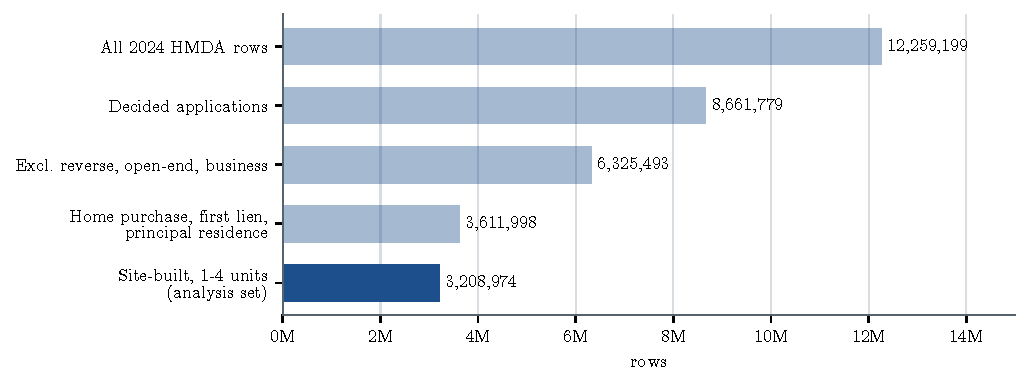
\includegraphics[width=0.85\linewidth]{fig_funnel.pdf}
  \caption{Cohort funnel. Each step gives the same count as the project proposal. We remove reverse mortgages, open-end lines of credit and business-purpose loans before the home-purchase filter.}
  \label{fig:funnel}
\end{figure}

The final set has \NRows{} rows.
The overall denial rate is \DenialRate{}.
The rate for each program is: Conventional \RateConv{}, FHA \RateFHA{}, VA \RateVA{} and USDA \RateUSDA{}.
A denial is a record with \code{action\_taken = 3}.
Originated applications count as not denied.
Approved applications that the applicant did not accept also count as not denied.

% ------------------------------------------------------------------ 2
\section{Method}
\subsection{Pipeline}
Both tools read the same split and the same feature definitions.
They join the data on a stored \code{row\_id}.
One script calculates all metrics from the saved test scores.
Thus no tool grades its own result.

\begin{figure}[H]
  \centering
  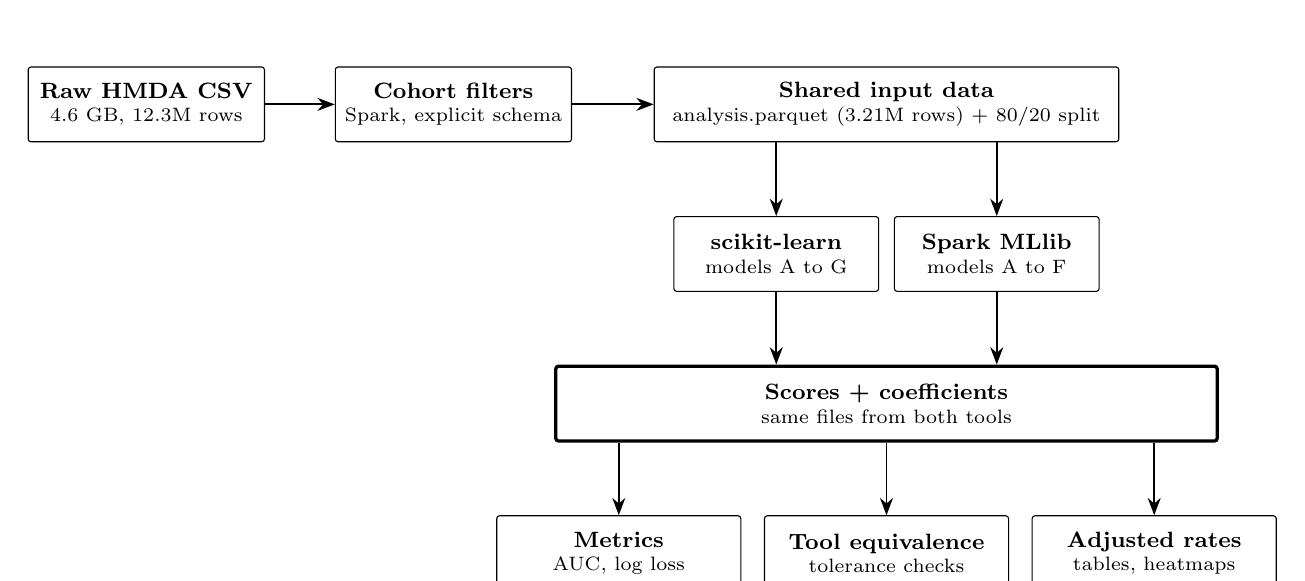
\begin{tikzpicture}[
      font=\footnotesize,
      box/.style={draw=black,fill=white,rounded corners=1pt,minimum width=3.0cm,minimum height=0.95cm,align=center,inner sep=2pt},
      wide/.style={box,minimum width=5.9cm},
      tool/.style={box,minimum width=2.6cm},
      outbox/.style={box,minimum width=3.1cm},
      key/.style={box,minimum width=8.4cm,line width=1.2pt},
      arr/.style={-{Stealth[length=2.2mm]},draw=black,line width=0.7pt}]
    \node[box]  (raw)  at (0,0)       {\textbf{Raw HMDA CSV}\\[-1pt]{\scriptsize 4.6 GB, 12.3M rows}};
    \node[box]  (coh)  at (3.9,0)     {\textbf{Cohort filters}\\[-1pt]{\scriptsize Spark, explicit schema}};
    \node[wide] (data) at (9.4,0)     {\textbf{Shared input data}\\[-1pt]{\scriptsize analysis.parquet (3.21M rows) + 80/20 split}};
    \node[tool] (sk)   at (8.0,-1.9)  {\textbf{scikit-learn}\\[-1pt]{\scriptsize models A to G}};
    \node[tool] (sp)   at (10.8,-1.9) {\textbf{Spark MLlib}\\[-1pt]{\scriptsize models A to F}};
    \node[key]  (sc)   at (9.4,-3.8)  {\textbf{Scores + coefficients}\\[-1pt]{\scriptsize same files from both tools}};
    \node[outbox]  (m1)   at (6.0,-5.7)  {\textbf{Metrics}\\[-1pt]{\scriptsize AUC, log loss}};
    \node[outbox]  (m2)   at (9.4,-5.7)  {\textbf{Tool equivalence}\\[-1pt]{\scriptsize tolerance checks}};
    \node[outbox]  (m3)   at (12.8,-5.7) {\textbf{Adjusted rates}\\[-1pt]{\scriptsize tables, heatmaps}};
    \draw[arr] (raw) -- (coh);
    \draw[arr] (coh) -- (data);
    \draw[arr] (sk.north |- data.south) -- (sk.north);
    \draw[arr] (sp.north |- data.south) -- (sp.north);
    \draw[arr] (sk.south) -- (sk.south |- sc.north);
    \draw[arr] (sp.south) -- (sp.south |- sc.north);
    \draw[arr] (m1.north |- sc.south) -- (m1.north);
    \draw[arr] (m2.north |- sc.south) -- (m2.north);
    \draw[arr] (m3.north |- sc.south) -- (m3.north);
  \end{tikzpicture}
  \caption{Pipeline. The raw data goes through the cohort filters to one set of input data with one split. Both tools read this set and write the same score files. The outputs are the metrics, the equivalence checks and the adjusted rates.}
  \label{fig:pipeline}
\end{figure}

\subsection{The model}
Let $y_i = 1$ if the lender denies application $i$.
Logistic regression gives the probability of denial as
\begin{equation}
  \pr(y_i = 1 \mid x_i) \;=\; \sigma(\beta_0 + x_i^{\top}\beta) \;=\; \frac{1}{1 + e^{-(\beta_0 + x_i^{\top}\beta)}} .
  \label{eq:logit}
\end{equation}
Each $x_i$ is a vector of 0/1 dummy columns and two standardized numbers.
Both tools use the same columns in the same order.
The predictors are loan type, \DTI{} bin, \CLTV{} bin, log income, an income-missing flag and log loan amount.
A missing \DTI{} or \CLTV{} value has its own bin.
We do not impute missing values.
Race, ethnicity, sex and age are not inputs.

Both tools minimize the same objective.
It has a small ridge penalty:
\begin{equation}
  \hat\beta \;=\; \argmin_{\beta_0,\beta}\; \frac{1}{n}\sum_{i=1}^{n}\Big[-y_i\log p_i-(1-y_i)\log(1-p_i)\Big] \;+\; \frac{\lambda}{2}\,\lVert\beta\rVert_2^{2},
  \qquad \lambda = 10^{-6}.
  \label{eq:objective}
\end{equation}
The intercept has no penalty.
scikit-learn uses $C = 1/(\lambda n)$.
Spark uses \code{regParam} $=\lambda$.
Thus the two objectives are the same.
We use no class weights.
Thus you can interpret the coefficients, and the probabilities stay calibrated.

\subsection{The model ladder}
\begin{table}[H]
  \centering
  \small
  \begin{tabular}{@{}p{6.4cm}ccccccc@{}}
\toprule
 & A & B & C & D & E & F & G \\
\midrule
Loan type, DTI bin, CLTV bin, log income, income-missing flag, log loan amount & \textcolor{navy}{$\bullet$} & \textcolor{navy}{$\bullet$} & \textcolor{navy}{$\bullet$} & \textcolor{navy}{$\bullet$} & \textcolor{navy}{$\bullet$} & \textcolor{navy}{$\bullet$} & \textcolor{navy}{$\bullet$} \\
DTI$\times$CLTV cross (rare cells pooled) &  & \textcolor{navy}{$\bullet$} & \textcolor{navy}{$\bullet$} & \textcolor{navy}{$\bullet$} & \textcolor{navy}{$\bullet$} & \textcolor{navy}{$\bullet$} &  \\
Loan type $\times$ DTI, loan type $\times$ CLTV &  &  & \textcolor{navy}{$\bullet$} & \textcolor{navy}{$\bullet$} & \textcolor{navy}{$\bullet$} & \textcolor{navy}{$\bullet$} &  \\
Finer DTI (each integer 36--49) &  &  &  & \textcolor{navy}{$\bullet$} &  &  &  \\
State dummies &  &  &  &  & \textcolor{navy}{$\bullet$} &  &  \\
Drop rows with CLTV above 150 &  &  &  &  &  & \textcolor{navy}{$\bullet$} &  \\
Learner & LR & LR & LR & LR & LR & LR & GBM \\
Fit in & sk+Sp & sk+Sp & sk+Sp & sk+Sp & sk+Sp & sk+Sp & sk \\
\bottomrule
\end{tabular}

  \caption{Model ladder. Model A is the baseline. Model B adds the \DTI{}$\times$\CLTV{} cross. Model C lets the \DTI{} and \CLTV{} effects change for each program. Models D, E and F are sensitivity tests with finer \DTI{} bins, state dummies, and no rows with a \CLTV{} above 150. Model G is a gradient-boosted tree model that shows if the logistic features miss structure.}
  \label{tab:ladder}
\end{table}

In Model C, the log-odds of denial is the sum of several terms.
The terms are a loan-type shift $\gamma_\ell$, a \DTI{}-bin shift $\delta_d$, a \CLTV{}-bin shift $\kappa_c$ and a joint-cell shift $\theta_{dc}$.
Two more terms, $\phi_{\ell d}$ and $\psi_{\ell c}$, give the program-specific shifts.
The model also has terms for the controls.
We pool the cells that have fewer than 500 train rows into one column, \code{other\_rare}.

\subsection{Adjusted denial rates}
We want to compare programs at each \DTI{} level and remove the effect of the other inputs.
For this, we use standardization.
Take the loans $S_\ell$ of program $\ell$.
Set the \DTI{} bin of each loan to $d$.
Keep the other features, predict, and calculate the average:
\begin{equation}
  \hat A_\ell(d) \;=\; \frac{1}{|S_\ell|}\sum_{i\in S_\ell}\hat p\big(x_i \text{ with \DTI{} bin set to } d\big).
  \label{eq:adjusted}
\end{equation}
We use the same method for the \CLTV{} bins.
The results show associations.
They do not show causes.

% ------------------------------------------------------------------ 3
\section{Prediction quality}
We calculate the metrics on the 20\% test split (\NTest{} rows, with \NTrain{} train rows).
ROC-AUC is the probability that a random denied loan has a higher score than a random approved loan.
PR-AUC is the average precision.
It gives more weight to the rare denied class.
A model with no skill has a PR-AUC that is equal to the denial rate, \BasePR{}.

Log loss and the Brier score show the quality of the probabilities.
The Brier score is $\frac{1}{n}\sum_i (p_i - y_i)^2$.
The intervals are 95\% bootstrap intervals from 200 resamples.

\begin{figure}[H]
  \centering
  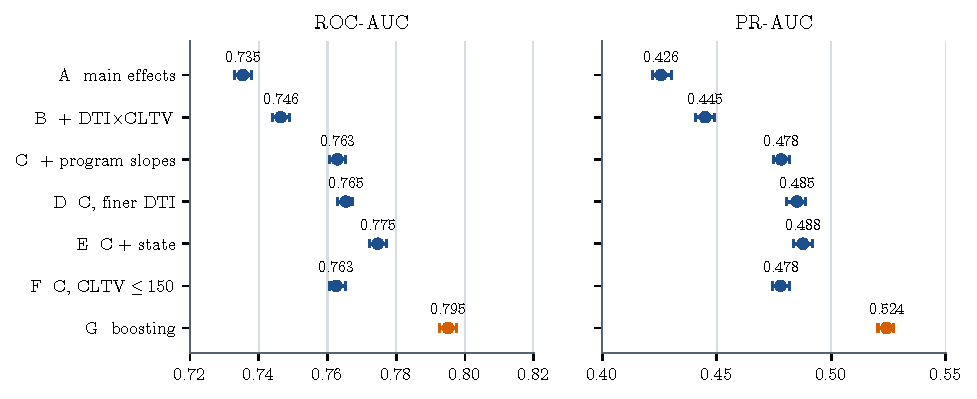
\includegraphics[width=\linewidth]{fig_metrics.pdf}
  \caption{ROC-AUC and PR-AUC with 95\% intervals. A higher value is better. A ROC-AUC of 0.5 is chance. The no-skill PR-AUC is \BasePR{}.}
  \label{fig:metrics}
\end{figure}

\begin{table}[H]
  \centering
  \small
  \begin{tabular}{@{}lrllrr@{}}
\toprule
Model & Columns & ROC-AUC [95\% CI] & PR-AUC [95\% CI] & Log loss & Brier \\
\midrule
Constant (train rate) & --- & 0.500 & 0.088 & 0.2986 & 0.0805 \\
\textbf{A}\ main effects & 16 & 0.735\,[0.733, 0.738] & 0.426\,[0.422, 0.430] & 0.2426 & 0.0635 \\
\textbf{B}\ + DTI$\times$CLTV & 51 & 0.746\,[0.744, 0.749] & 0.445\,[0.441, 0.449] & 0.2378 & 0.0621 \\
\textbf{C}\ + program slopes & 81 & 0.763\,[0.761, 0.765] & 0.478\,[0.475, 0.482] & 0.2289 & 0.0593 \\
\textbf{D}\ C, finer DTI & 221 & 0.765\,[0.763, 0.767] & 0.485\,[0.481, 0.489] & 0.2273 & 0.0588 \\
\textbf{E}\ C + state & 135 & 0.775\,[0.772, 0.777] & 0.488\,[0.484, 0.492] & 0.2262 & 0.0587 \\
\textbf{F}\ C, CLTV$\leq$150 & 81 & 0.763\,[0.761, 0.765] & 0.478\,[0.474, 0.482] & 0.2286 & 0.0592 \\
\textbf{G}\ boosting & --- & 0.795\,[0.793, 0.798] & 0.524\,[0.520, 0.527] & 0.2170 & 0.0563 \\
\bottomrule
\end{tabular}

  \caption{Test-set metrics for all models (scikit-learn).}
  \label{tab:metrics}
\end{table}

Each step from Model A to B to C increases both metrics.
The bootstrap intervals do not overlap.
State dummies (Model E) increase the ROC-AUC by approximately \EGain{} over Model C.
The finer \DTI{} bins (Model D) and the removal of the \CLTV{} rows above 150 (Model F) give almost no change.
Model G is better than Model C by \Gap{} PR-AUC.
This is more than the limit of 0.02 in the plan.

\subsection{Results for each program}
\begin{table}[H]
  \centering
  \small
  \begin{tabular}{@{}lrrcccccc@{}}
\toprule
 & & & \multicolumn{2}{c}{Model A} & \multicolumn{2}{c}{Model C} & \multicolumn{2}{c}{Model G} \\
\cmidrule(lr){4-5}\cmidrule(lr){6-7}\cmidrule(lr){8-9}
Program & Test rows & Denied & ROC & PR & ROC & PR & ROC & PR \\
\midrule
Conventional & 429\,553 & 7.7\% & 0.755 & 0.448 & 0.760 & 0.480 & 0.802 & 0.529 \\
FHA & 136\,629 & 12.5\% & 0.703 & 0.463 & 0.721 & 0.491 & 0.759 & 0.545 \\
VA & 68\,087 & 8.2\% & 0.685 & 0.274 & 0.705 & 0.285 & 0.728 & 0.368 \\
USDA & 7\,526 & 12.2\% & 0.702 & 0.401 & 0.718 & 0.428 & 0.767 & 0.496 \\
\bottomrule
\end{tabular}

  \caption{ROC-AUC and PR-AUC in each loan program, for Models A, C and G.}
  \label{tab:byprogram}
\end{table}

Each model ranks Conventional loans highest and VA loans lowest.
VA loans have the lowest AUC for all three models.
Thus \DTI{} and \CLTV{} explain less of the denials for VA loans.

\begin{table}[H]
  \centering
  \small
  \begin{tabular}{@{}lrlrr@{}}
\toprule
Model B fit in one program & Test rows & ROC-AUC [95\% CI] & PR-AUC & Log loss \\
\midrule
Conventional & 429\,553 & 0.763\,[0.760, 0.766] & 0.481 & 0.2026 \\
FHA & 136\,629 & 0.724\,[0.719, 0.728] & 0.499 & 0.2940 \\
VA & 68\,087 & 0.700\,[0.692, 0.709] & 0.317 & 0.2489 \\
USDA & 7\,526 & 0.718\,[0.700, 0.737] & 0.428 & 0.3089 \\
\bottomrule
\end{tabular}

  \caption{Model B fitted in each program alone. This is an alternative to program interaction terms.}
  \label{tab:progb}
\end{table}

USDA has approximately 7\,500 test rows.
Thus its interval is wide.

\subsection{Calibration}
\begin{figure}[H]
  \centering
  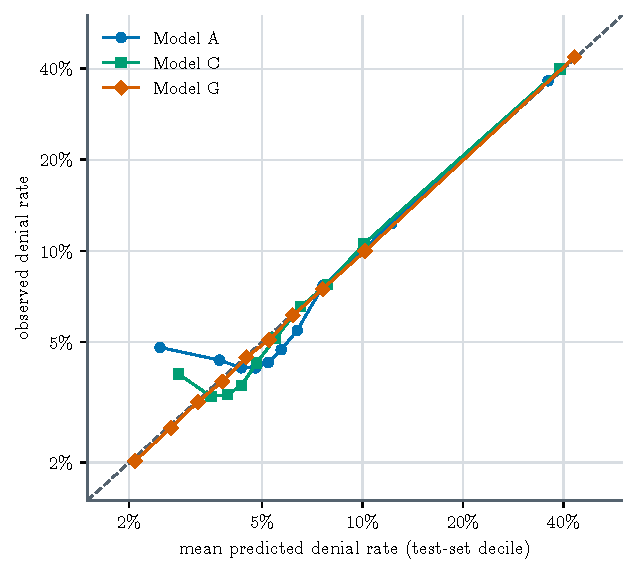
\includegraphics[width=0.62\linewidth]{fig_calibration.pdf}
  \caption{Predicted and observed denial rate for each decile of the test set, on logarithmic axes. Nine of the ten deciles have a predicted rate of 12.2\% or less. A point on the dashed line shows perfect calibration. Model A predicts too low in the lowest decile and too high in the middle deciles. Model C has a largest gap of approximately 1 point. Model G has a largest gap of 0.5 points.}
  \label{fig:calibration}
\end{figure}

% ------------------------------------------------------------------ 4
\section{Effect of \DTI{} and \CLTV{}}
\subsection{Model A: odds ratios}
\begin{figure}[H]
  \centering
  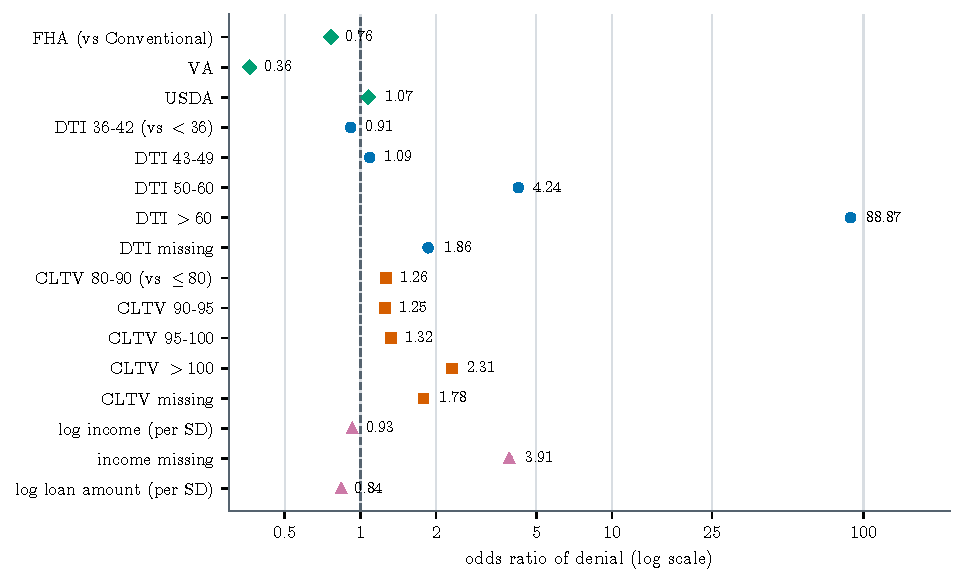
\includegraphics[width=0.82\linewidth]{fig_forest.pdf}
  \caption{Odds ratios of denial for Model A, with 95\% intervals. The reference levels are Conventional, \DTI{} below 36 and \CLTV{} 80 or less. The colors and marker shapes show the groups: green diamond for loan type, blue circle for \DTI{}, orange square for \CLTV{} and pink triangle for the controls. We calculate the standard errors from the Fisher information.}
  \label{fig:forest}
\end{figure}

An odds ratio of 1 means no change.
A \DTI{} above 60 multiplies the odds of denial by \ORDtiHigh{}.
A \DTI{} of 50--60 multiplies them by \ORDtiMid{}.
These values are against a \DTI{} below 36.
A \CLTV{} above 100 multiplies the odds by \ORCltvHigh{}.

After the controls, the odds for a VA loan are \ORVA{} times the odds for a Conventional loan.
The odds for an application with no income are \ORIncome{} times higher.
Thus a missing value carries information.

The odds ratio is $\mathrm{OR}_j = e^{\beta_j}$.
The 95\% interval is $\exp(\hat\beta_j \pm 1.96\,\mathrm{se}_j)$.
We calculate the variance as
\begin{equation}
  \Var(\hat\beta) \;\approx\; \big(X^{\top}WX + n\lambda I_0\big)^{-1}, \qquad W = \operatorname{diag}\big(\hat p_i(1-\hat p_i)\big).
\end{equation}
Model A uses one \DTI{} effect for all programs.
This is too limited, as the next figures show.

\subsection{Adjusted denial rate by \DTI{} (Model C)}
\begin{figure}[H]
  \centering
  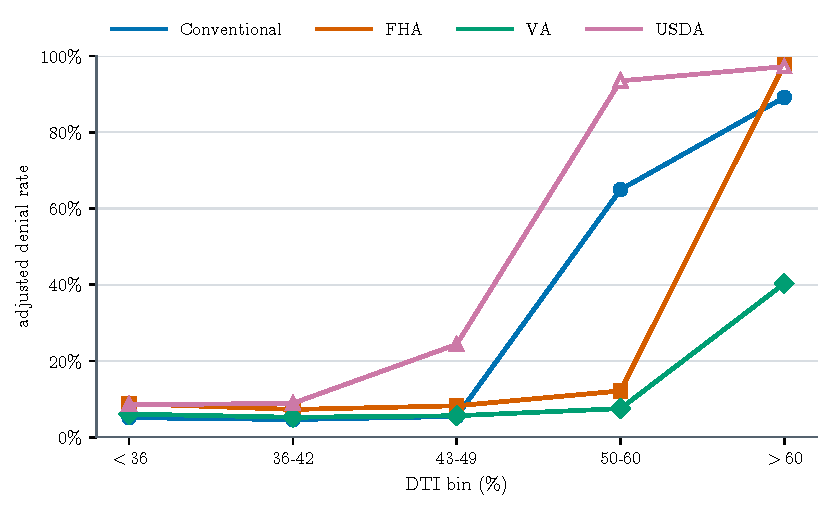
\includegraphics[width=0.82\linewidth]{fig_dti.pdf}
  \caption{Adjusted denial rate by \DTI{} bin. The limit is at \DTI{} 50--60 for Conventional and USDA loans. It is above \DTI{} 60 for FHA and VA loans. The USDA points at 50--60 and above 60 have approximately 425 loans each (hollow markers). The plot does not show the missing-\DTI{} bin.}
  \label{fig:dti}
\end{figure}

Conventional loans have a denial rate of approximately 5\% up to \DTI{} 49.
In the 50--60 bin, the rate is \DtiConvHigh{}.
FHA and VA loans have low rates at \DTI{} 50--60 (\DtiFhaMid{} and \DtiVaMid{}).
Above \DTI{} 60, the rates are \DtiFhaHigh{} and \DtiVaHigh{}.
The USDA rate increases earlier, at \DTI{} 43--49 (\DtiUsdaLow{} to \DtiUsdaMid{}).

The data has no lender rules and no credit scores.
Thus the model cannot show the reason for these steps.
HMDA gives \DTI{} as integers only from 36 to 49.
All other values are in wide bins.
Thus we cannot find the limits more accurately.

\subsection{Adjusted denial rate by \CLTV{} (Model C)}
\begin{figure}[H]
  \centering
  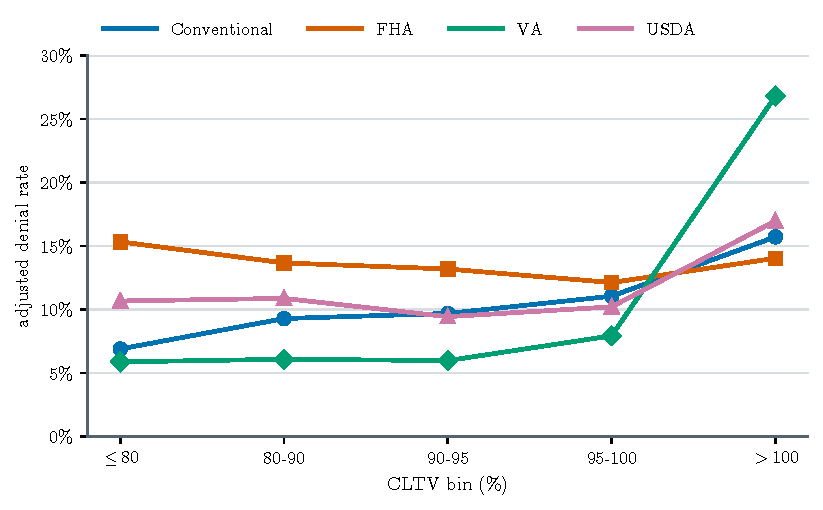
\includegraphics[width=0.82\linewidth]{fig_cltv.pdf}
  \caption{Adjusted denial rate by \CLTV{} bin. The effects are small below 100\%. Above 100\%, the rate increases for Conventional and VA loans. The vertical axis stops at 30\%. Most FHA loans are in the 95--100 bin. Thus the other FHA bins have few loans and the curve is irregular.}
  \label{fig:cltv}
\end{figure}

\subsection{\DTI{}$\times$\CLTV{} together (Model B)}
\begin{figure}[H]
  \centering
  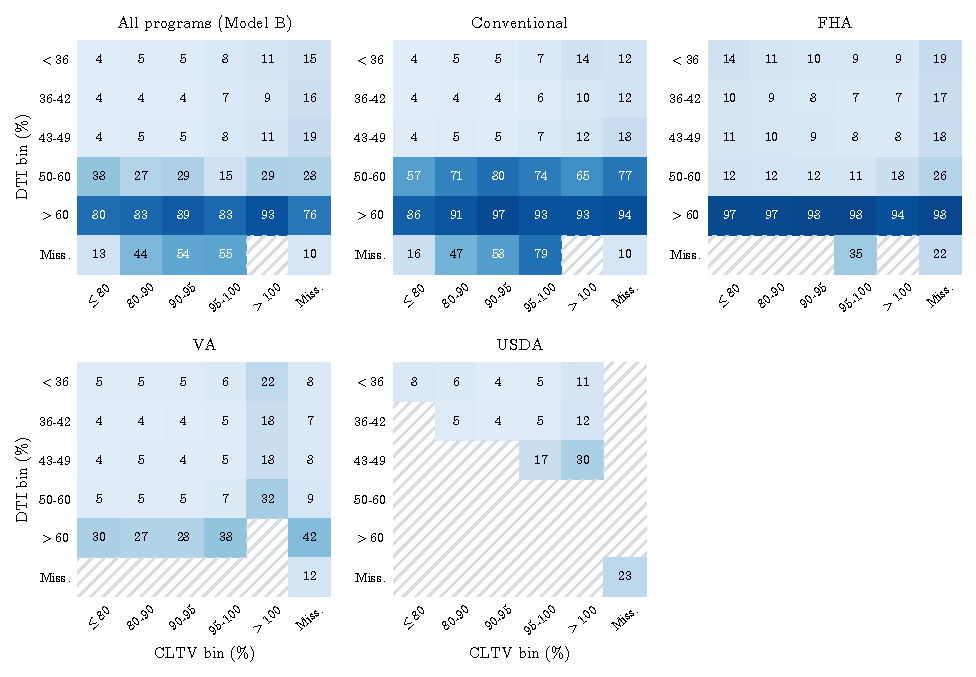
\includegraphics[width=\linewidth]{fig_heat.pdf}
  \caption{Adjusted denial rate (\%) over \DTI{}$\times$\CLTV{}. A dark cell shows a higher rate. A hatched cell has fewer than 500 observed loans. We mask these cells. The first panel shows Model B on all loans, and the other panels show Model B fitted in each program alone. \DTI{} is the main axis in each panel.}
  \label{fig:heat}
\end{figure}

\subsection{First bin with a large rise}
\begin{table}[H]
  \centering
  \small
  \begin{tabular}{@{}llcr@{}}
\toprule
Variable & Program & First bin with a rise above 5 pp & Rise (pp) \\
\midrule
DTI & Conventional & 50-60 & +60 \\
DTI & FHA & $>$60 & +86 \\
DTI & VA & $>$60 & +33 \\
DTI & USDA & 43-49 & +15 \\
CLTV & Conventional & none & --- \\
CLTV & FHA & none & --- \\
CLTV & VA & $>$100 & +19 \\
CLTV & USDA & $>$100 & +7 \\
\bottomrule
\end{tabular}

  \caption{First bin where the adjusted rate of Model C is more than 5 percentage points above the previous bin. This is a description. It is not a statistical test.}
  \label{tab:thresholds}
\end{table}

The rule finds no \CLTV{} rise for Conventional or FHA loans.

% ------------------------------------------------------------------ 5
\section{Comparison of the two tools}\label{sec:tools}
The central comparison of the project is Pandas/scikit-learn against Spark MLlib.
We use the same data and the same model in both.
The plan gives tolerances for the coefficients, the intercept, the test ROC-AUC, the log loss and the score correlation.

\begin{table}[H]
  \centering
  \footnotesize
  \begin{tabular}{@{}lllllll@{}}
\toprule
Model & Max coef.\ diff. & Intercept diff. & ROC-AUC diff. & Log loss diff. & Score corr. & Iter.\ sk / Spark \\
\midrule
\textbf{A} & 4.6e-05 \textcolor{okgreen}{pass} & 4.3e-06 \textcolor{okgreen}{pass} & 4.7e-08 \textcolor{okgreen}{pass} & 3.0e-09 \textcolor{okgreen}{pass} & 1.000000 \textcolor{okgreen}{pass} & 44 / 25 \\
\textbf{B} & 1.6e-01 \textcolor{badred}{\textbf{fail}} & 6.5e-05 \textcolor{okgreen}{pass} & 7.7e-07 \textcolor{okgreen}{pass} & 9.2e-09 \textcolor{okgreen}{pass} & 1.000000 \textcolor{okgreen}{pass} & 159 / 149 \\
\textbf{C} & 1.9e-01 \textcolor{badred}{\textbf{fail}} & 3.0e-04 \textcolor{okgreen}{pass} & 7.2e-08 \textcolor{okgreen}{pass} & 6.5e-08 \textcolor{okgreen}{pass} & 1.000000 \textcolor{okgreen}{pass} & 377 / 200 \\
\bottomrule
\end{tabular}

  \caption{Equivalence of scikit-learn and Spark. Each cell shows the absolute difference and the result against the tolerance. The tolerances are $10^{-3}$ for the coefficients and the intercept, $10^{-4}$ for ROC-AUC and log loss, and a correlation of at least 0.9999.}
  \label{tab:equiv}
\end{table}

Model A passes all checks.
For Models B and C, all checks on the predictions pass.
Only the coefficient check does not pass.
The largest differences are 0.16 and 0.19, and the tolerance is $10^{-3}$.

\medskip
\noindent\fcolorbox{black}{white}{\parbox{\dimexpr\linewidth-2\fboxsep-2\fboxrule\relax}{%
\small\raggedright
\textbf{Cause of the coefficient difference in Models B and C.}
\par\smallskip
Models B and C have the \DTI{} main effects, the \CLTV{} main effects and the full \DTI{}$\times$\CLTV{} cross.
These columns are collinear.
For each \DTI{} bin $d$, the sum of the cells in that bin is equal to the indicator of that bin:
\begin{equation*}
  \sum_{c}\indic[\mathrm{DTI}=d,\ \mathrm{CLTV}=c] \;=\; \indic[\mathrm{DTI}=d].
\end{equation*}
Thus many sets of coefficients give the same predictions.
Only the ridge penalty of $10^{-6}$ selects one set.
The two tools stop at different points along a flat direction.
The differences are equal and opposite between a main effect and its cell dummy.
\par\smallskip
Spark also stopped at its limit of 200 iterations for Models C, D, E and F.
Thus it did not reach the tolerance of $10^{-7}$.
A higher limit can decrease the gap for Model C.
We did not test this.
\par\smallskip
We did not change the tolerances or the results.
To read Models B and C, use the adjusted rates.
They do not depend on how the tool divides the redundant weight.}}

\medskip
The fit times for Model A were \FitASk{} s (scikit-learn) and \FitASp{} s (Spark).
For Model C they were \FitCSk{} s and \FitCSp{} s.
Each value is from one run on a laptop.
Spark cached its input.
These values are not a benchmark.

% ------------------------------------------------------------------ 6
\section{Limits}
\begin{itemize}
  \item \textbf{Associations, not causes.} The data has no credit score, assets, employment history or lender rules.
  \item \textbf{No application date.} We split the data at random, with strata of denial and loan type. The split is not by time.
  \item \textbf{Missing \DTI{} and \CLTV{} values are not random.} Conventional loans with a missing \DTI{} have a denial rate of approximately 15\%. FHA loans have approximately 34\%. Each missing value has its own bin.
  \item \textbf{\DTI{} is coarse.} HMDA gives integers only from 36 to 49.
  \item \textbf{USDA has few loans.} Each of its two highest \DTI{} bins has approximately 425 loans. Treat these estimates as weak.
  \item \textbf{The models do not use protected attributes.} This report does not test for disparate impact.
  \item \textbf{We inferred the cohort filters.} The filters for principal residence and 1--4 units give the same counts as the proposal. The proposal text does not state them.
  \item \textbf{We did not do two optional items.} These are the fit-time benchmark and the Spark fits for each program alone.
\end{itemize}

\vfill
\hrule\vspace{0.5em}
{\footnotesize
Source: FFIEC HMDA 2024 national loan-level dataset.
The code, results and tests are in the \texttt{mortgage-analysis} project.
The script \texttt{report/build\_latex.py} makes each number, table and figure from \texttt{results/*.csv}.
We wrote the text with the rules of Simplified Technical English (ASD-STE100) and with technical names.
This is not an official ASD check.}

\end{document}
